%%%%%%%%%%%%%%%%%%%%%%%%%%%%%%%%%%%%%%%%%
% Jacobs Landscape Poster
% LaTeX Template
% Version 1.1 (14/06/14)
%
% Created by:
% Computational Physics and Biophysics Group, Jacobs University
% https://teamwork.jacobs-university.de:8443/confluence/display/CoPandBiG/LaTeX+Poster
% 
% Further modified by:
% Nathaniel Johnston (nathaniel@njohnston.ca)
%
% This template has been downloaded from:
% http://www.LaTeXTemplates.com
%
% License:
% CC BY-NC-SA 3.0 (http://creativecommons.org/licenses/by-nc-sa/3.0/)
%
%%%%%%%%%%%%%%%%%%%%%%%%%%%%%%%%%%%%%%%%%

%----------------------------------------------------------------------------------------
%	PACKAGES AND OTHER DOCUMENT CONFIGURATIONS
%----------------------------------------------------------------------------------------

\documentclass[final]{beamer}

\usepackage[scale=1.24]{beamerposter} % Use the beamerposter package for laying out the poster

\usetheme{confposter} % Use the confposter theme supplied with this template

\setbeamercolor{block title}{fg=ngreen,bg=white} % Colors of the block titles
\setbeamercolor{block body}{fg=black,bg=white} % Colors of the body of blocks
\setbeamercolor{block alerted title}{fg=white,bg=dblue!70} % Colors of the highlighted block titles
\setbeamercolor{block alerted body}{fg=black,bg=dblue!10} % Colors of the body of highlighted blocks
% Many more colors are available for use in beamerthemeconfposter.sty

%-----------------------------------------------------------
% Define the column widths and overall poster size
% To set effective sepwid, onecolwid and twocolwid values, first choose how many columns you want and how much separation you want between columns
% In this template, the separation width chosen is 0.024 of the paper width and a 4-column layout
% onecolwid should therefore be (1-(# of columns+1)*sepwid)/# of columns e.g. (1-(4+1)*0.024)/4 = 0.22
% Set twocolwid to be (2*onecolwid)+sepwid = 0.464
% Set threecolwid to be (3*onecolwid)+2*sepwid = 0.708

\newlength{\sepwid}
\newlength{\onecolwid}
\newlength{\twocolwid}
\newlength{\threecolwid}
\setlength{\paperwidth}{48in} % A0 width: 46.8in
\setlength{\paperheight}{36in} % A0 height: 33.1in
\setlength{\sepwid}{0.024\paperwidth} % Separation width (white space) between columns
\setlength{\onecolwid}{0.22\paperwidth} % Width of one column
\setlength{\twocolwid}{0.464\paperwidth} % Width of two columns
\setlength{\threecolwid}{0.708\paperwidth} % Width of three columns
\setlength{\topmargin}{-0.5in} % Reduce the top margin size
%-----------------------------------------------------------

\usepackage{graphicx}  % Required for including images

\usepackage{booktabs} % Top and bottom rules for tables

%----------------------------------------------------------------------------------------
%	TITLE SECTION 
%----------------------------------------------------------------------------------------

\title{QUANTUM ANNEALING COMPARISION ON DIFFERENT QPU} % Poster title

\author{Dhruvil Gandhi} % Author(s)

\institute{Seidenberg School of CSIS, Pace University} % Institution(s)

%----------------------------------------------------------------------------------------

\begin{document}

\addtobeamertemplate{block end}{}{\vspace*{2ex}} % White space under blocks
\addtobeamertemplate{block alerted end}{}{\vspace*{2ex}} % White space under highlighted (alert) blocks

\setlength{\belowcaptionskip}{2ex} % White space under figures
\setlength\belowdisplayshortskip{2ex} % White space under equations

\begin{frame}[t] % The whole poster is enclosed in one beamer frame

\begin{columns}[t] % The whole poster consists of three major columns, the second of which is split into two columns twice - the [t] option aligns each column's content to the top

\begin{column}{\sepwid}\end{column} % Empty spacer column

\begin{column}{\onecolwid} % The first column

%----------------------------------------------------------------------------------------
%	OBJECTIVES
%----------------------------------------------------------------------------------------

\begin{alertblock}{Objectives}

The goals of this research project is to:
\begin{itemize}
\item Understand different approaches of quantum computing.
\item Understand the concept of quantum annealing and hybrid quantum computation.
\item Implement integer factoring on different quantum computing systems. 
\item Try to compare the results
\end{itemize}

\end{alertblock}

%----------------------------------------------------------------------------------------
%	INTRODUCTION
%----------------------------------------------------------------------------------------

\begin{block}{Introduction}

    Quantum computing is an up and coming technology which has gained a lot of potential and advancement in recent times. With companies like IBM, D-Wave, Google etc. allowing public access to quantum computing resources and limitation on different approaches, there are numerous different algorithms and use cases that can be implemented and quantum supremacy over classical computing be achieved. I accessed different platforms and approaches of quantum computing. Since gate based quantum computing has limited number of quantum bits or qubits, I was particularly interested in quantum annealing approach. 

    I researched the math of quantum annealing and implement it on D-Wave and Rigetti Systems quantum computer.

\end{block}

%------------------------------------------------

\begin{figure}

\includegraphics[width=0.8\linewidth]{uqc.png}
\caption{Universal Quantum Computer}
\end{figure}

%----------------------------------------------------------------------------------------

\end{column} % End of the first column

\begin{column}{\sepwid}\end{column} % Empty spacer column

\begin{column}{\twocolwid} % Begin a column which is two columns wide (column 2)

\begin{columns}[t,totalwidth=\twocolwid] % Split up the two columns wide column

\begin{column}{\onecolwid}\vspace{-.6in} % The first column within column 2 (column 2.1)

%----------------------------------------------------------------------------------------
%	MATERIALS
%----------------------------------------------------------------------------------------

\begin{block}{Universal Quantum Computer}

A universal quantum computer is one where gate model approach can be mapped to other approaches in polynomial time. Various approaches to quantum computing are:

\begin{itemize}
\item Gate Based
\item Measurement Based
\item Topological
\item Adiabatic
\end{itemize}

D-Wave works on adiabatic quantum computing using quantum annealing. It has 2038 qubits. 

Rigetti's quantum computer works on gate based model and has a comcept of lattice, where a lattice is connected qubits which can go upto 18. 



\end{block}

%----------------------------------------------------------------------------------------

\end{column} % End of column 2.1

\begin{column}{\onecolwid}\vspace{-.6in} % The second column within column 2 (column 2.2)

%----------------------------------------------------------------------------------------
%	METHODS
%----------------------------------------------------------------------------------------

\begin{block}{Quantum Annealing}

In quantum annealing, we simulate the problem and all possible outcomes for a given problem are calculated. The soultion is based on minima of the nenrgy graph of the quantum system. To provide bias, magnetic fields are applied, this bias being the constraints we want our solution to satisfy.

Quantum annealing uses hamiltonian framework, the system must remain in ground state during simulation and operation. Hamiltomian framework is given by:
\begin{multline*}
    \mathcal{H}_s(s) = \frac{-1}{2} \sum_i \Delta (s) \sigma_i^x   + \epsilon(s) ( - \sum_i h_i \sigma_i^z + \sum_{i<j} J_{ij}  \sigma_i^z \sigma_j^z)
\end{multline*}


\end{block}

%----------------------------------------------------------------------------------------

\end{column} % End of column 2.2

\end{columns} % End of the split of column 2 - any content after this will now take up 2 columns width

%----------------------------------------------------------------------------------------
%	IMPORTANT RESULT
%----------------------------------------------------------------------------------------

\begin{alertblock}{Important Result}

On D-Wave, the results were observed, after 20 runs, the results were at different energy levels, though consistent in terms of factors. 

Hybrid approach on Rigetti was not finished.

\end{alertblock} 

%----------------------------------------------------------------------------------------

\begin{columns}[t,totalwidth=\twocolwid] % Split up the two columns wide column again

\begin{column}{\onecolwid} % The first column within column 2 (column 2.1)



\begin{block}{D-Wave}

For adiabatic quantum computing using quantum annealing, integer factoring was implemented based on D-Wave using their example sample given on LEAP. 

\begin{enumerate}
\item Formulate the problem as constraint satisfaction problem.
\item Convert the model to binary quabratic model
\item Run on quantum processing unit.
\item Observe the results for factoring from 1 to 61.
\end{enumerate}
  
\begin{figure}
    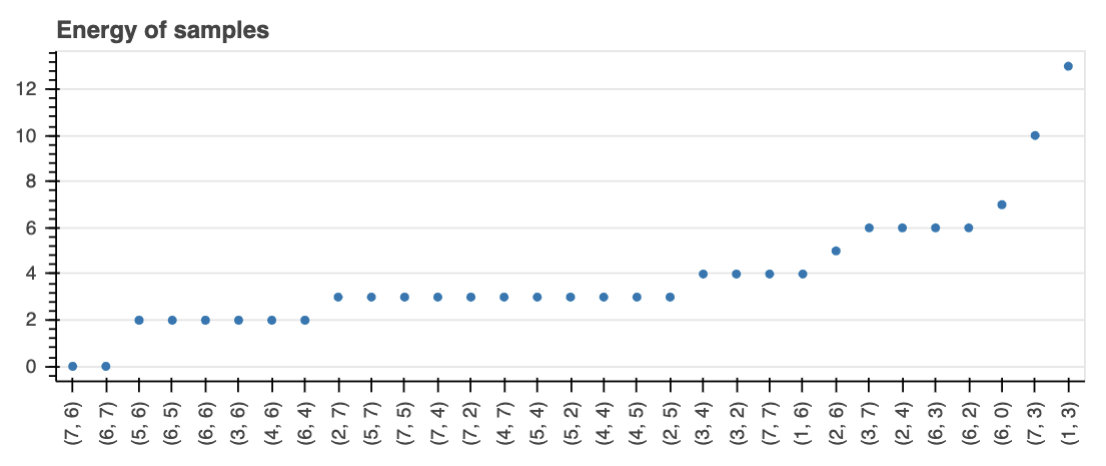
\includegraphics[width=0.8\linewidth]{dwaveresult.png}
    \caption{D-Wave result for a large number}
    \end{figure}

\end{block}

%----------------------------------------------------------------------------------------

\end{column} % End of column 2.1

\begin{column}{\onecolwid} % The second column within column 2 (column 2.2)

%----------------------------------------------------------------------------------------
%	RESULTS
%----------------------------------------------------------------------------------------

\begin{block}{Rigetti}


On Rigetti, using their FOrest SDK and pyquil, the implementation was not finised. The figure below shows solution graph for a sample problem on Rigetti.
\begin{figure}
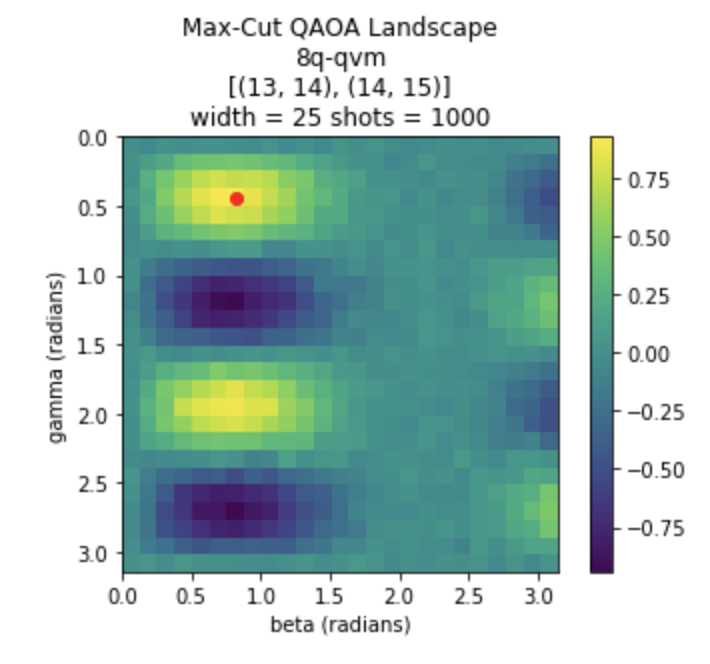
\includegraphics[width=0.8\linewidth]{rigettisampler.png}
\caption{Sample Rigetti result}
\end{figure}

\end{block}


%----------------------------------------------------------------------------------------

\end{column} % End of column 2.2

\end{columns} % End of the split of column 2

\end{column} % End of the second column

\begin{column}{\sepwid}\end{column} % Empty spacer column

\begin{column}{\onecolwid} % The third column

%----------------------------------------------------------------------------------------
%	CONCLUSION
%----------------------------------------------------------------------------------------

\begin{block}{Gates for Quantum Computer}

\begin{figure}
    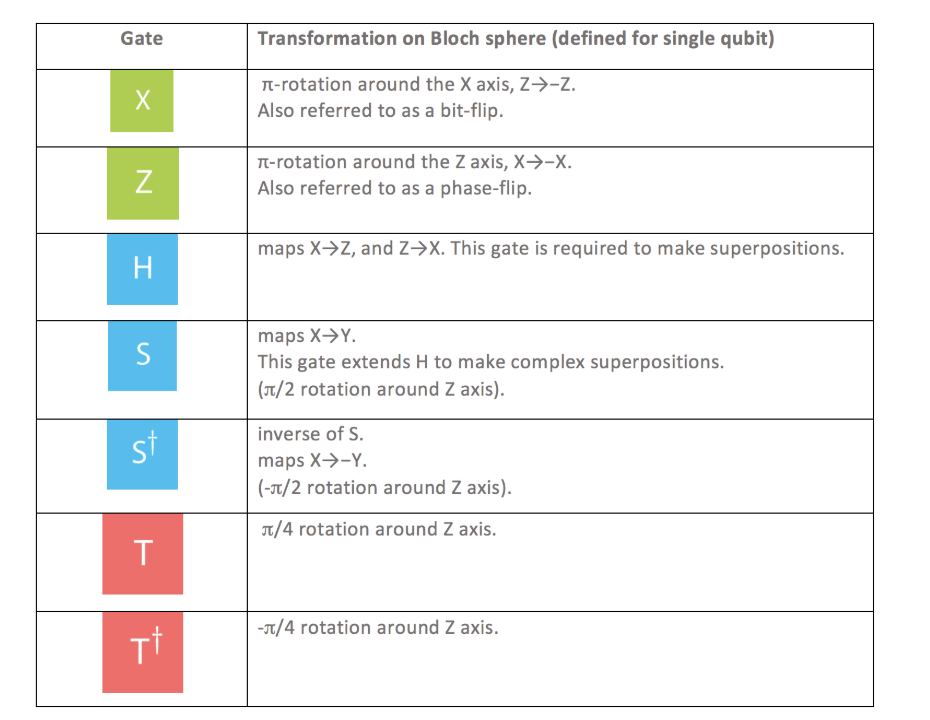
\includegraphics[width=0.8\linewidth]{gates.png}
    \caption{Quantum Computing Gates}
    \end{figure}
    

\end{block}

%----------------------------------------------------------------------------------------
%	ADDITIONAL INFORMATION
%----------------------------------------------------------------------------------------

\begin{block}{Additional Information}

Maecenas ultricies feugiat velit non mattis. Fusce tempus arcu id ligula varius dictum. 
\begin{itemize}
\item Curabitur pellentesque dignissim
\item Eu facilisis est tempus quis
\item Duis porta consequat lorem
\end{itemize}

\end{block}


%----------------------------------------------------------------------------------------
%	ACKNOWLEDGEMENTS
%----------------------------------------------------------------------------------------

\setbeamercolor{block title}{fg=red,bg=white} % Change the block title color

\begin{block}{Acknowledgements}

\small{\rmfamily{Special thanks to Dr. Juan Shan, Dr. Charles Tappert, Dr. Ronald Frank, Dr. Stephan Barabasi and Rigetti's team(for providing access and credits to the system).}} \\

\end{block}

%----------------------------------------------------------------------------------------
%	CONTACT INFORMATION
%----------------------------------------------------------------------------------------

\setbeamercolor{block alerted title}{fg=black,bg=norange} % Change the alert block title colors
\setbeamercolor{block alerted body}{fg=black,bg=white} % Change the alert block body colors

\begin{alertblock}{Contact Information}

\begin{itemize}
\item Web: \href{http://github.com/dhruv857}{http://github.com/dhruv857}
\item Email: \href{mailto:jdgandhi@pace.edu}{dgandhi@gace.edu}
\end{itemize}

\end{alertblock}

\begin{center}
\begin{tabular}{ccc}

\includegraphics[width=0.4\linewidth]{seidenberg.jpg} 
\end{tabular}
\end{center}

%----------------------------------------------------------------------------------------

\end{column} % End of the third column

\end{columns} % End of all the columns in the poster

\end{frame} % End of the enclosing frame

\end{document}
